\documentclass{report}
\usepackage[utf8]{inputenc}
\usepackage{amsfonts}
\usepackage{mathtools}
\usepackage{amsmath}
\usepackage{arydshln}
\usepackage{algpseudocode}
\usepackage{algorithm}
\usepackage{algorithmicx}
\usepackage{changepage}
\usepackage{float}
\usepackage{graphicx}
\usepackage[makeroom]{cancel}
\usepackage{tikz}
\usepackage[english]{babel}
\usepackage{amsthm}
\usepackage{theoremref}
\usepackage{wrapfig}
\usepackage{caption}

\newtheorem{definition}{Definition}[section]
\newtheorem{proposition}{Proposition}[section]
\newtheorem{lemma}{Lemma}[section]
\newtheorem{theorem}{Theorem}[section]

\title{Dinic's Algorithm}
\author{Ian Orzel, Grant Butler, Josh Temel}
\date{April 2022}

\begin{document}

\maketitle

\tableofcontents

\section{Abstract}

\chapter{The Max Flow Problem}
A graph is a common tool utilized by computer scientists and mathematicians to study many different phenomenon. There are many different types of graphs, but we examine a unique case of them in this paper, which we call a network. These graphs are directed, weighted, and have a defined source and sink node.

We will try to build some intuition on what is implied by a network. The simplest analogy is to visualize a network of pipes. The edges in the network are pipes, and the vertices are junction points of pipes. Rather than visualizing the "weights" of edges as weights, we call these capacities. These represent the maximum flow that can be sent down a pipe. Then, in the network, we define the source as an infinite source of water and the sink as an infinite reserve for water.

Then, one can imagine flow being sent through the network. Flow is sent from the source and ends up in the sink. At each node other than the source and the sink, the amount of flow input into the node equals the amount of flow that is output. One can imagine the flow as water being sent through the network of pipes. Hence, the flow value is the amount of flow that has been sent through the network.

Now, we can define the problem of interest that we wish to solve through this project. What is the maximum amount of flow that we can send through this network from the source to the sink. The algorithm, Dinic's algorithm, attempts to find the max flow of an arbitrary network.

\chapter{Historical Solution}
Although this paper will focus on an analysis of Dinic's algorithm, there are other proposed algorithms that solve the max flow problem. Two of them that will be discussed in this section are the Ford-Fulkerson algorithm and the Edmonds-Karp algorithm. Although these also solve the max flow problem, their time complexities are worse when compared to Dinic's algorithm. With that being said, a lot of the ideas of Dinic's algorithm are reflected in the other two algorithms. Becuase these algorithms are much simplier to understand than Dinic's algorithm, we will spend some time discussing them in order to help bridge into the algorithm.

\section{Ford-Fulkerson}
The Ford-Fulkerson algorithm is a very basic algorithm to solve the max flow problem. It operates on the simple idea of picking an arbitrary path from the source to the sink, sending flow down the path, and updating the graph repeatedly until the source became disconnected from the sink. Some these steps seem a little ambiguous, so we will provide some minor description of how they operate.

The idea of picking an arbitrary path from the source to the sink is obvious, so we first focus on sending flow down the path. This is done by finding the edge on the path with the smallest capacity. This value will be the amount of flow that is sent down the path. This flow value is stored, as the max flow of the graph will be the sum of all of these flow values.

Next, the graph will need to be updated along this path. First, each edge along the path will have its capacity decreased by the amount of flow that was just sent along the path. Then, we need to define a back edge of an edge in a network, which is a corresponding edge that points in the opposite direction. During the update process, the back edges of every edge in the path will be increased by the amount of flow sent along the path.

This process continues until the source is disconnected from the sink. In this case, a blocking flow has been reached, which means that the corresponding flow is the max flow of the network. There is more information about this fact in the mathematical analysis.

The algorithm has a time complexity of $O(|E|*f)$, where $|E|$ is the number of edges in the network and $f$ is the max flow of the network. We can clearly see that this algorithm is not ideal, as we generally do not want the time complexity of an algorithm to be a function of the value being computed. It is for this reason that the Edmonds-Karp algorithm improves upon the shortcomings of Ford-Fulkerson.

\section{Edmonds-Karp}
The Edmonds-Karp algorithm operates similarly to the Ford-Folkerson algorithm, but there is one major difference between the two. While Ford-Folkerson chooses an arbitrary path to send the flow down for each iteration, Edmonds-Karp instead chooses the shortest path as found by breadth-first search (BFS). One must be careful when stating "shortest" path, as, although the graph is weighted, this shortest path does not take into account the weights of the edges. Instead, this shortest path is defined by the number of edges included in the path between the two nodes. Hence, Edmonds-Karp finds a shortest path between the source and sink, and it sends flow down this path.

Beyond this fact, Ford-Fulkerson and Edmonds-Karp are identical. So why does there exist a separate name for this seemingly very similar algorithm. This differnce can be seen in the time complexity, as Edmonds-Karp has complexity of $O(|V||E|^2)$, were $|V|$ is the number of vertices in the network and $|E|$ is the number of edges in the network. Now, we posit that Edmonds-Karp has a "better" time complexity than Ford-Fulkerson, but this is not the most obvious statement. Ford-Fulkerson is unique in the fact that its time complexity is a function of the value it is computing. So, if this value is very small, Ford-Fulkerson runs much faster than Edmonds-Karp. But, in a more general case where the max flow can be arbitrary large (which it is often assumed to be), Edmonds-Karp runs in much faster time (as it is a special case of Ford-Fulkerson).

\chapter{Dinic's Algorithm}
\section{Description of Dinic's}
The purpose of Dinic's Algorithm is to solve the max flow problem in a much faster time complexity than other solutions. It performs in $O\left(V^{2}E\right)$ time, which is much faster than the Ford-Fulkerson or Edmonds-Karp algorithms. Dinic's starts in a similar way to Edmonds-Karp, and uses BFS to find the level of each node in the graph. Then, multiple DFSs are used to find paths from the source to the sink, where the only valid paths are ones that go from level $L$ to $L + 1$. The capacity of the edges are then updated based on the bottleneck value through the path. This is repeated until a blocking flow is reached, where no more flow can be sent from the source to the sink. Adding up all bottleneck value values renders the maximum flow through the graph.

\pagebreak

\section{Visualization of Dinic's}

\begin{figure}[!htb]
    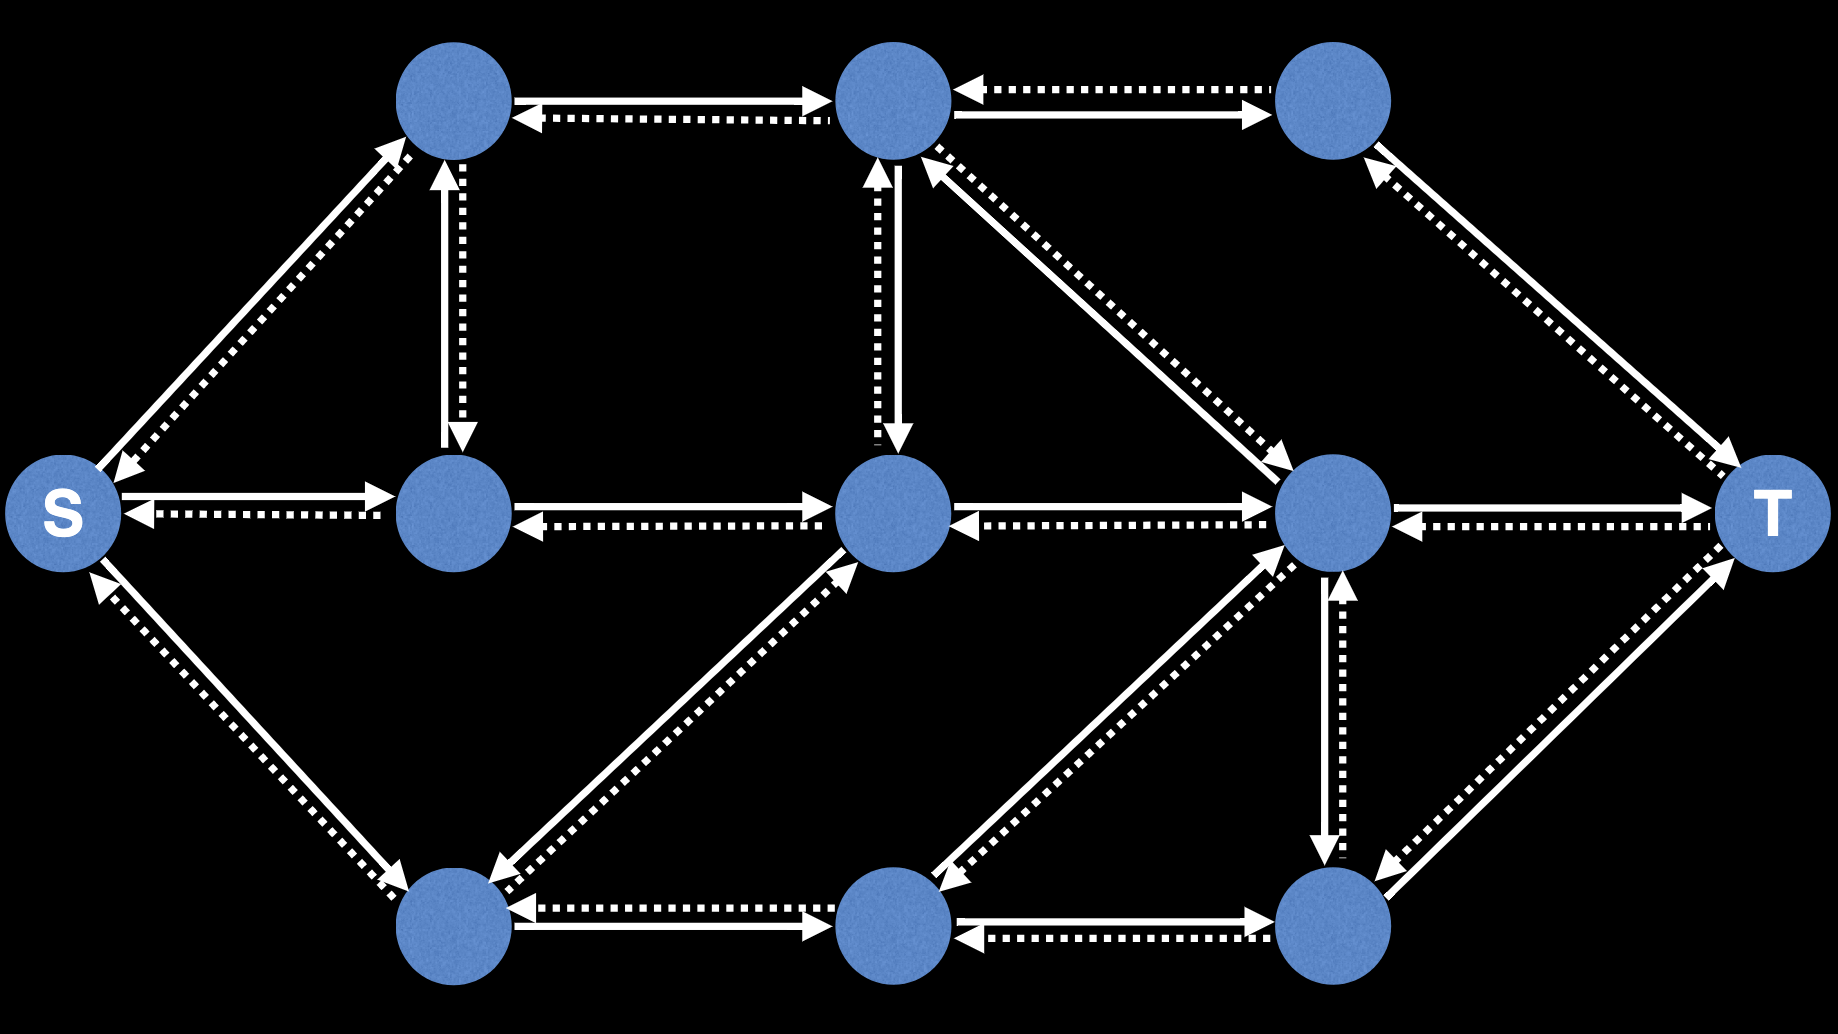
\includegraphics[width=\textwidth]{assets/visual01.png}
    \centering
    \captionsetup{justification=centering,margin=2cm}
    \caption{Graph \textit{G} with nodes \textit{s} (source) and \textit{t} (sink).}
\end{figure}
\begin{figure}[!htb]
    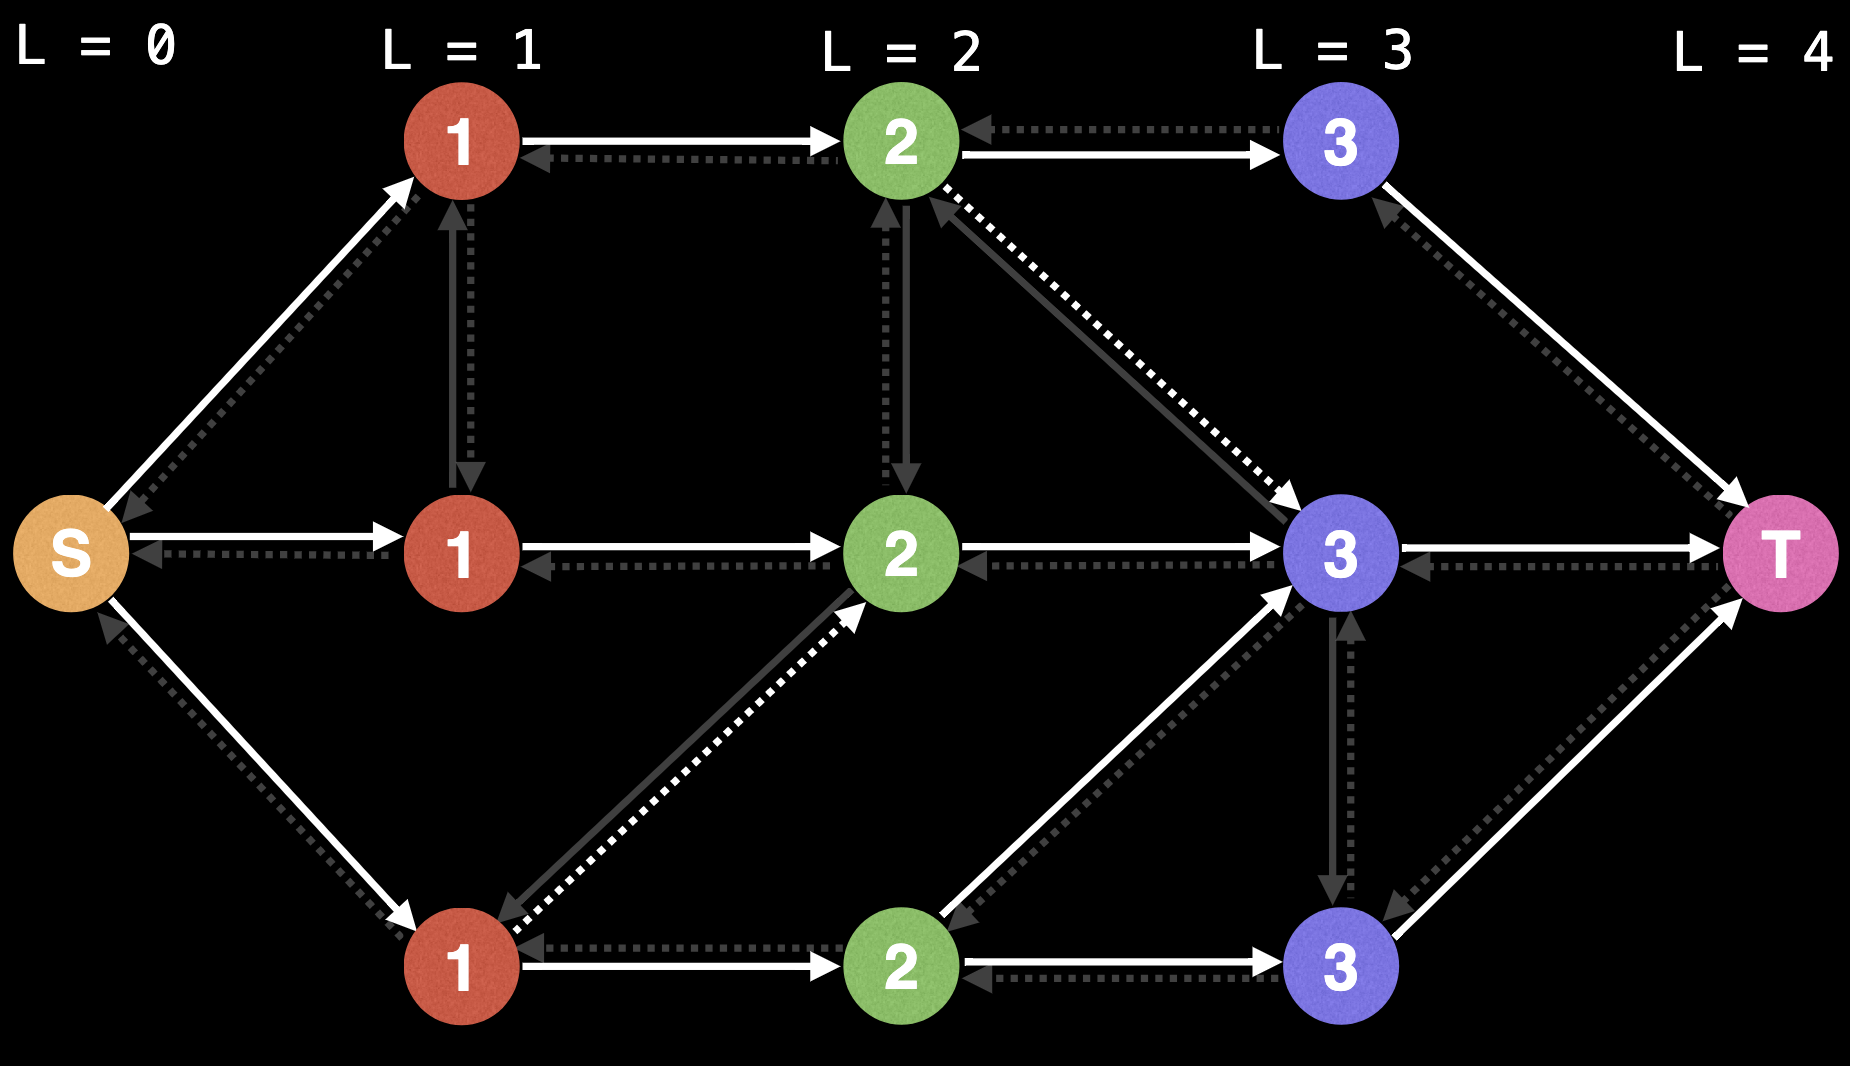
\includegraphics[width=\textwidth]{assets/visual02.png}
    \centering
    \captionsetup{justification=centering,margin=2cm}
    \caption{Marked levels after running \textit{BFS(G, s)}}
\end{figure}
\pagebreak
\begin{figure}[!htb]
    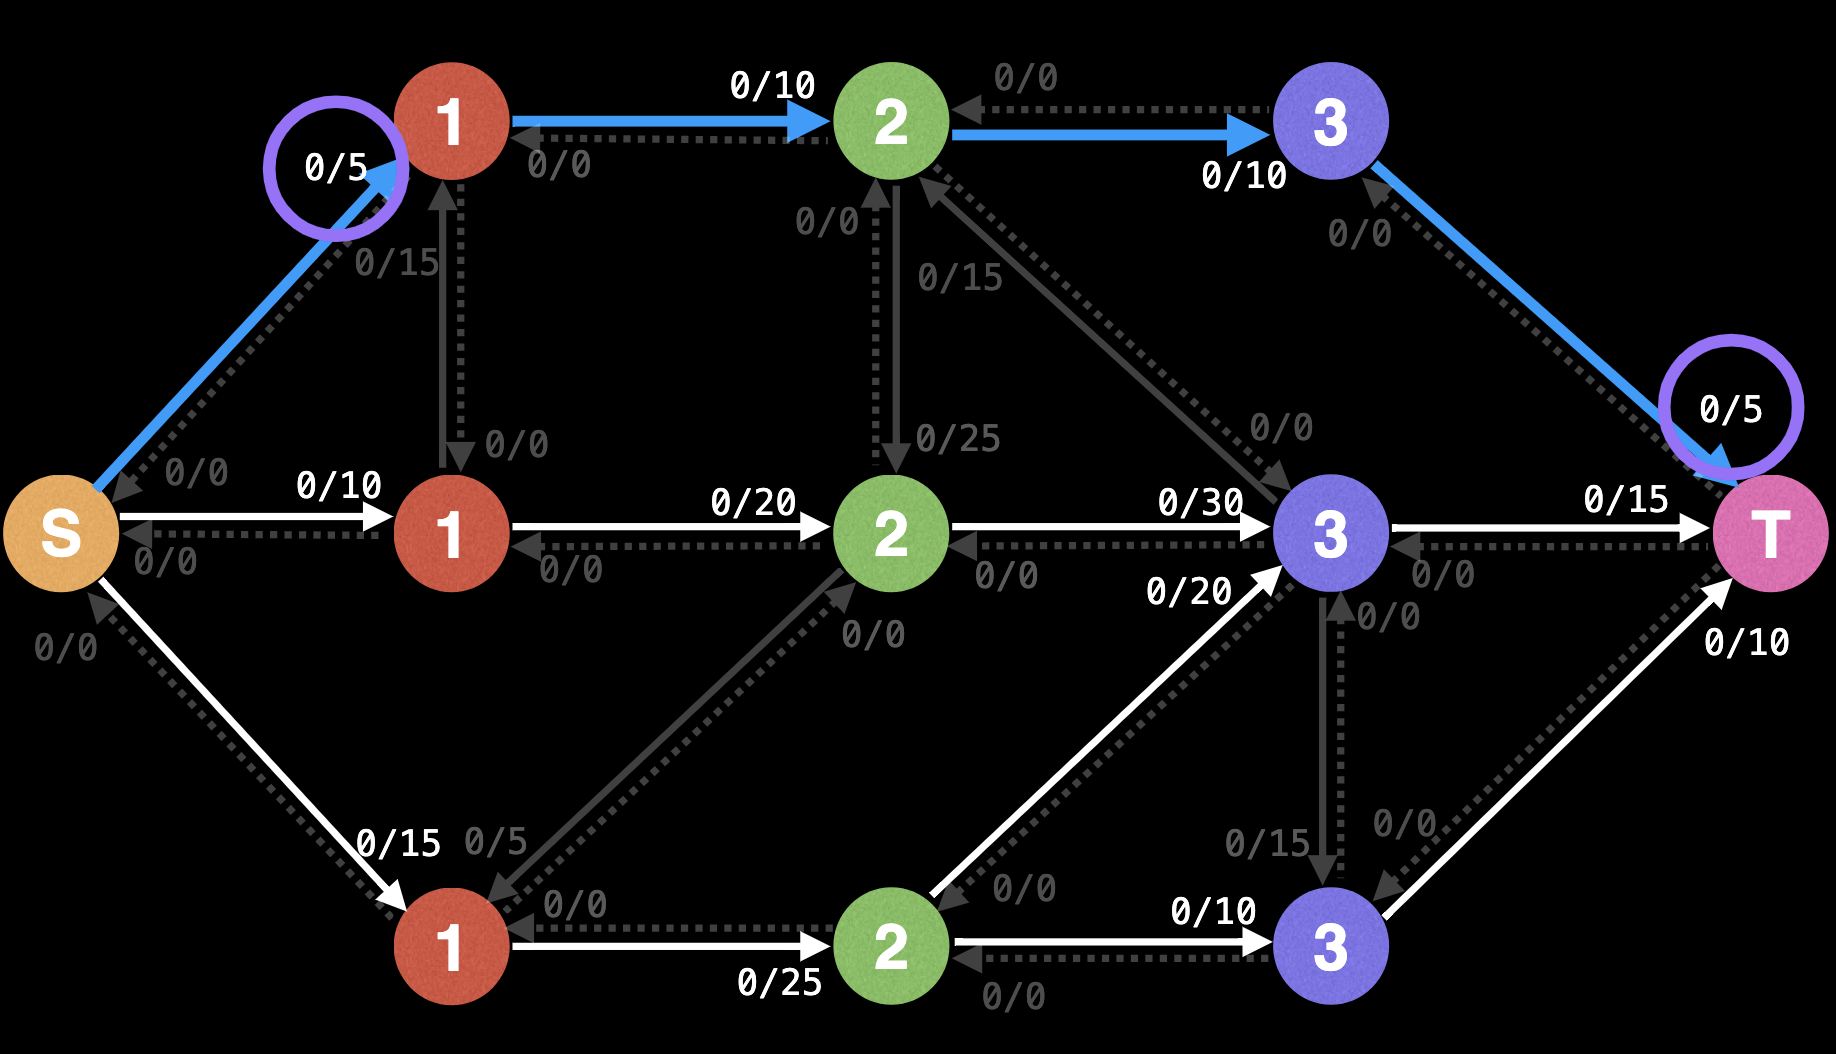
\includegraphics[width=\textwidth]{assets/visual03.png}
    \centering
    \captionsetup{justification=centering,margin=2cm}
    \caption{Path found using \textit{DFS(G, s, t, $\infty$)}, marking \textbf{bottleneck value} of the path.}
\end{figure}
\begin{figure}[!htb]
    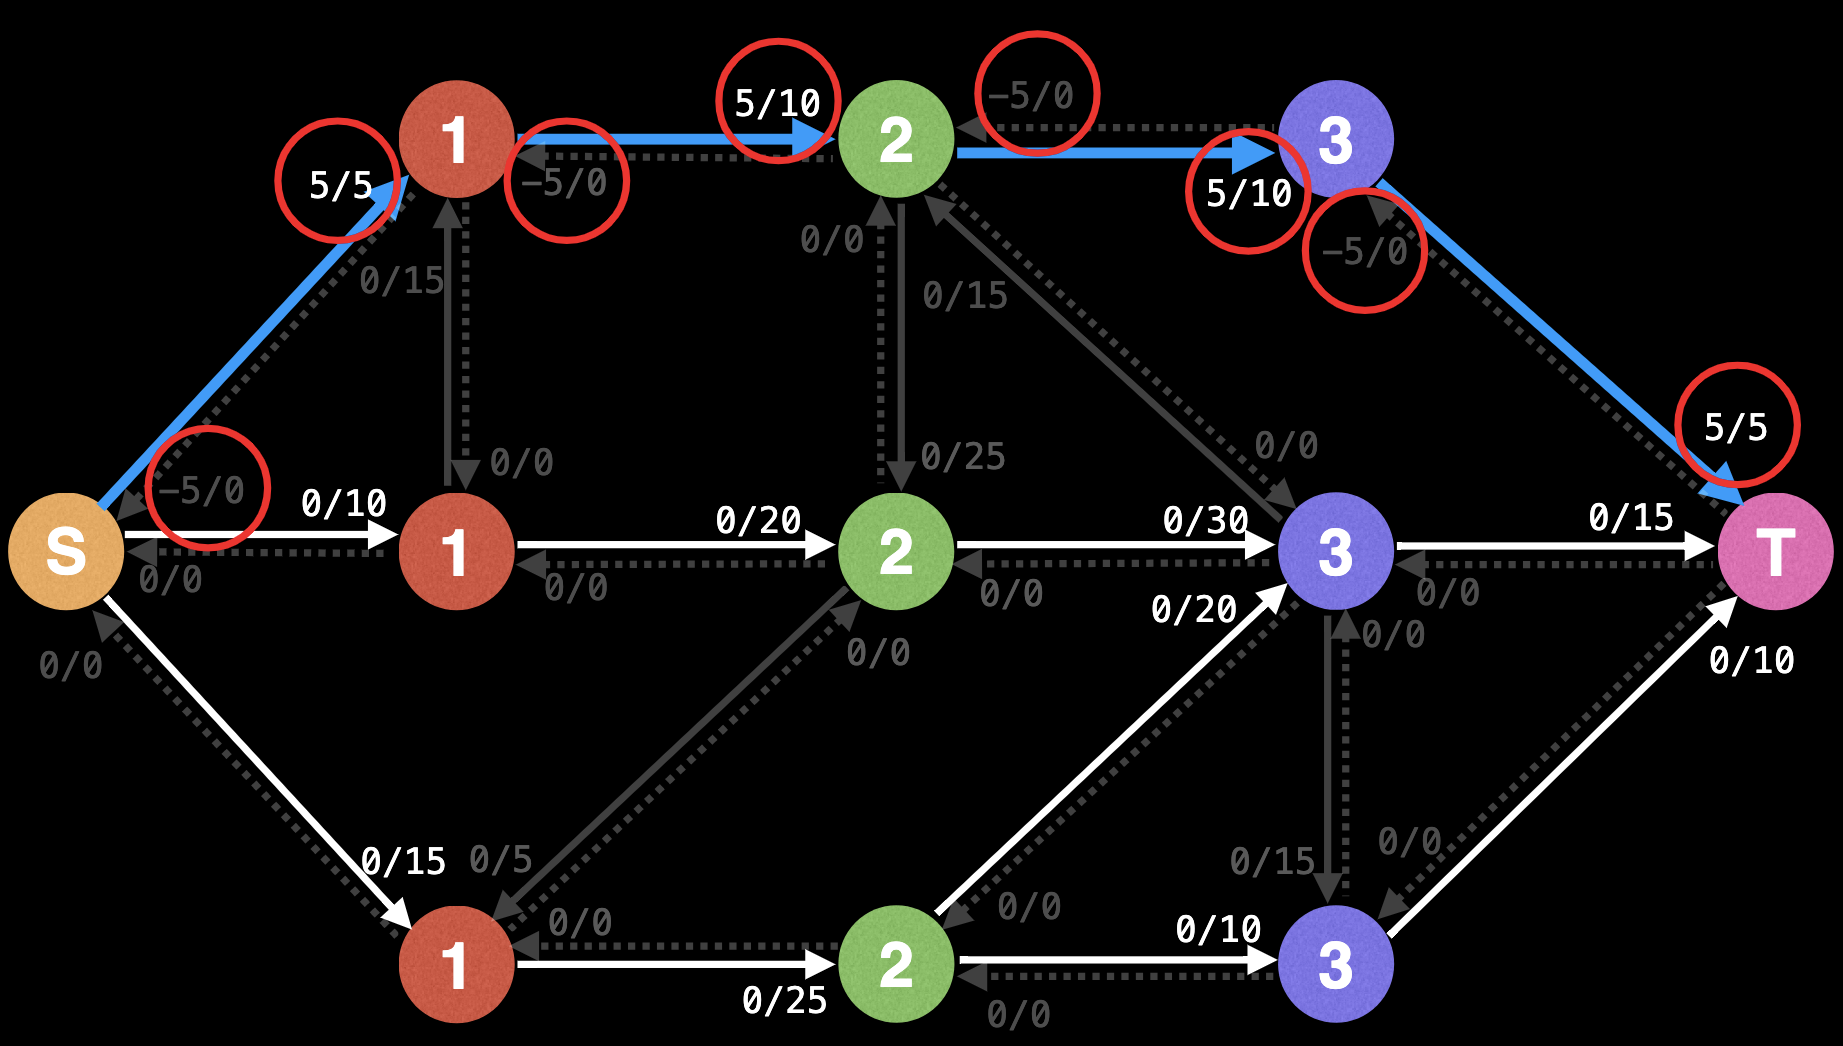
\includegraphics[width=\textwidth]{assets/visual04.png}
    \centering
    \captionsetup{justification=centering,margin=2cm}
    \caption{Augmenting the flow values on the path with \textbf{bottleneck value}.}
\end{figure}
\pagebreak
\begin{figure}[!htb]
    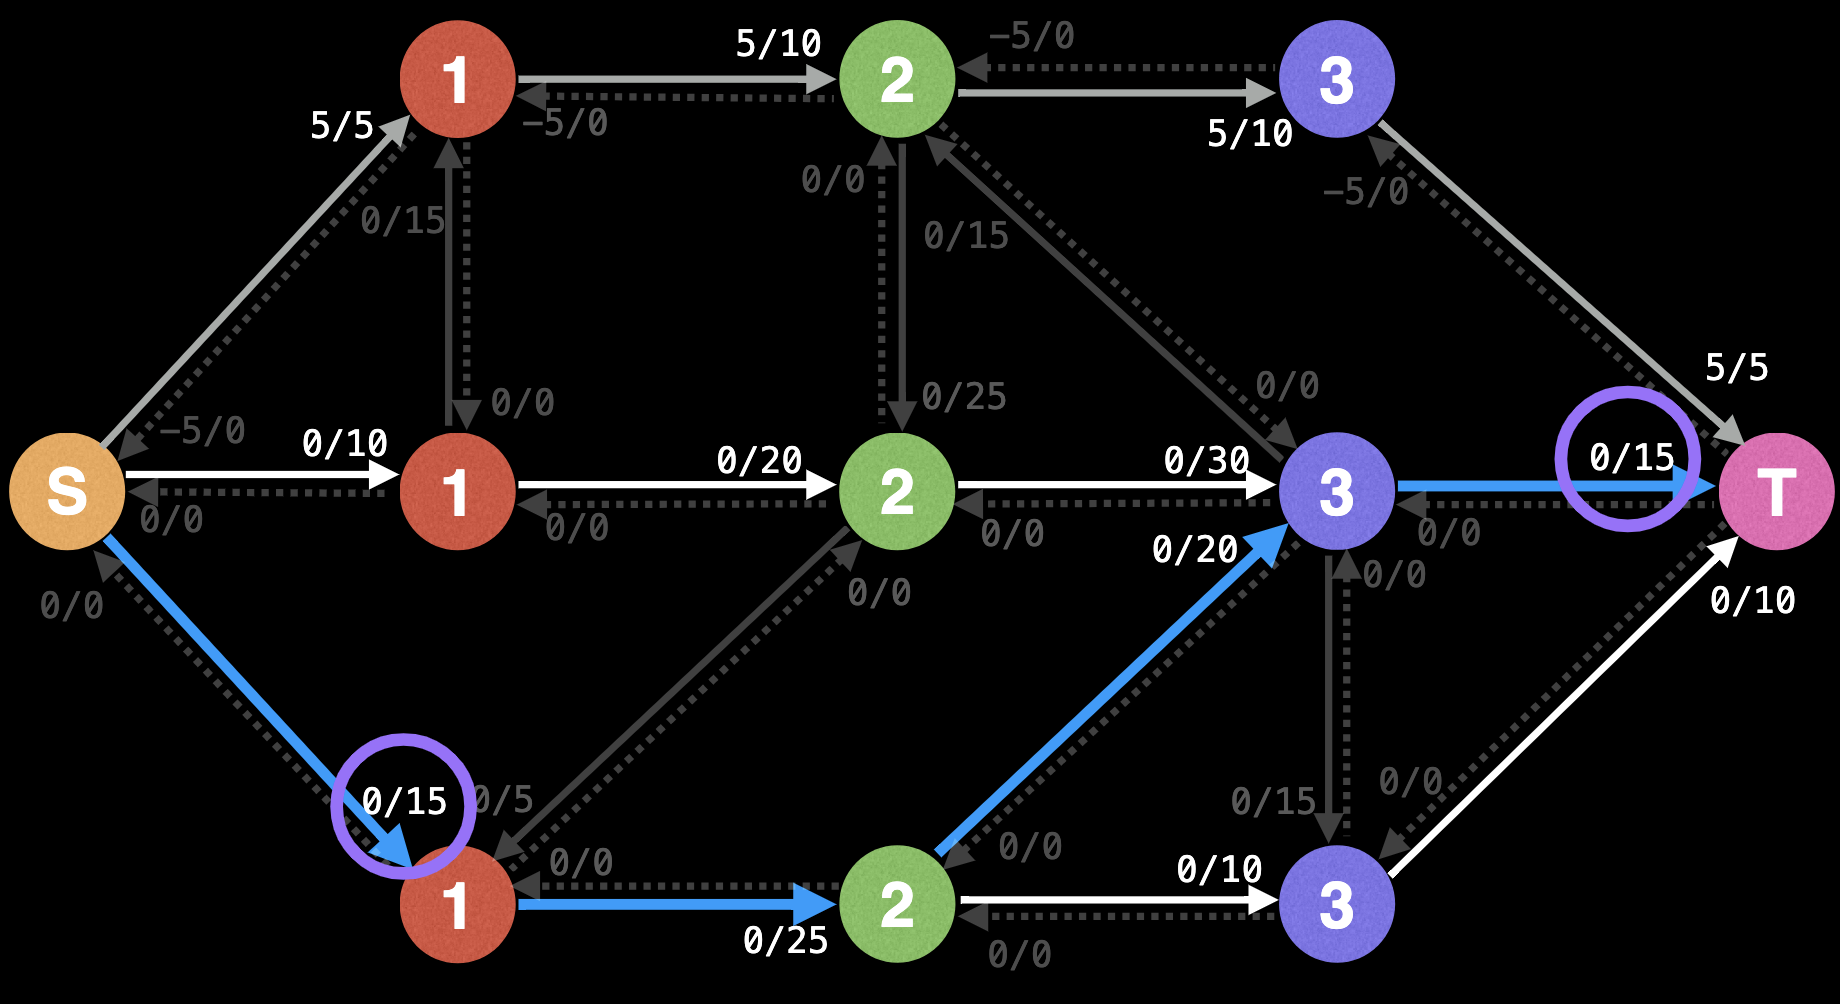
\includegraphics[width=\textwidth]{assets/visual05.png}
    \centering
    \captionsetup{justification=centering,margin=2cm}
    \caption{Another path found using \\\textit{DFS(G, s, t, $\infty$)}.}
\end{figure}
\begin{figure}[!htb]
    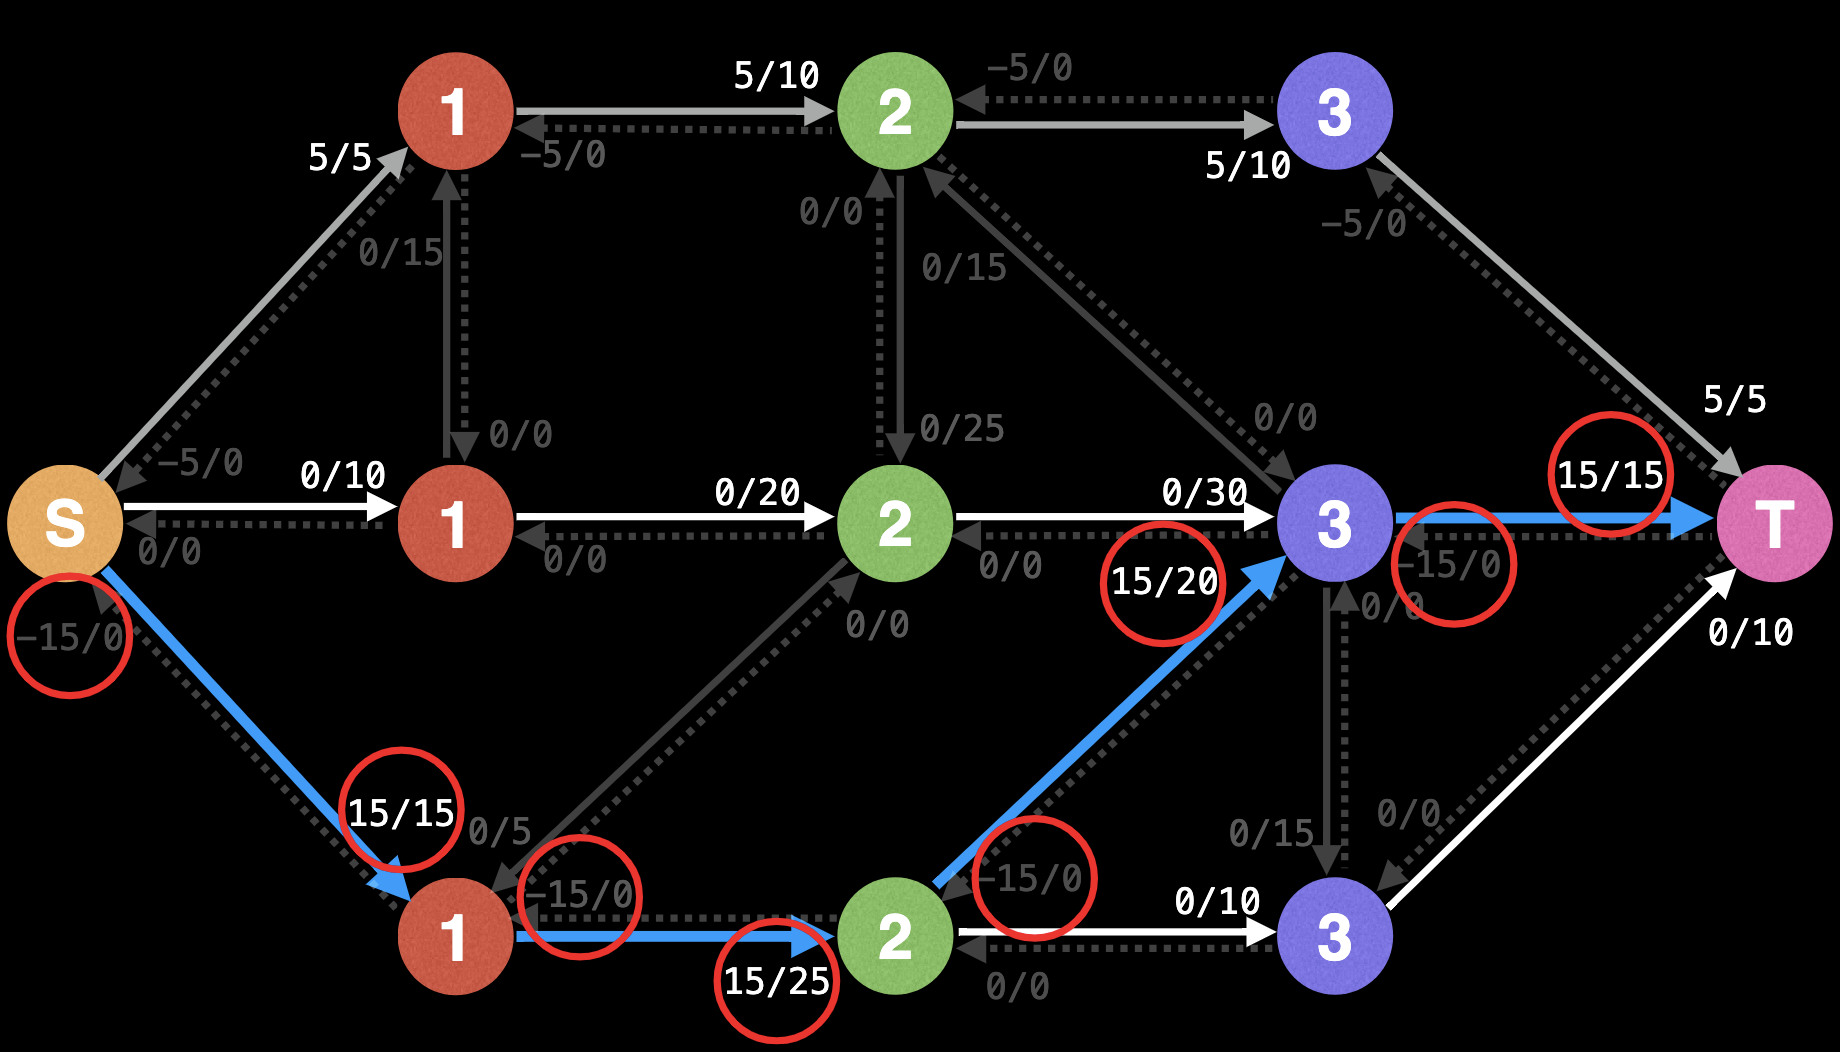
\includegraphics[width=\textwidth]{assets/visual06.png}
    \centering
    \captionsetup{justification=centering,margin=2cm}
    \caption{Augmented flow values on the path.}
\end{figure}
\pagebreak
\begin{figure}[!htb]
    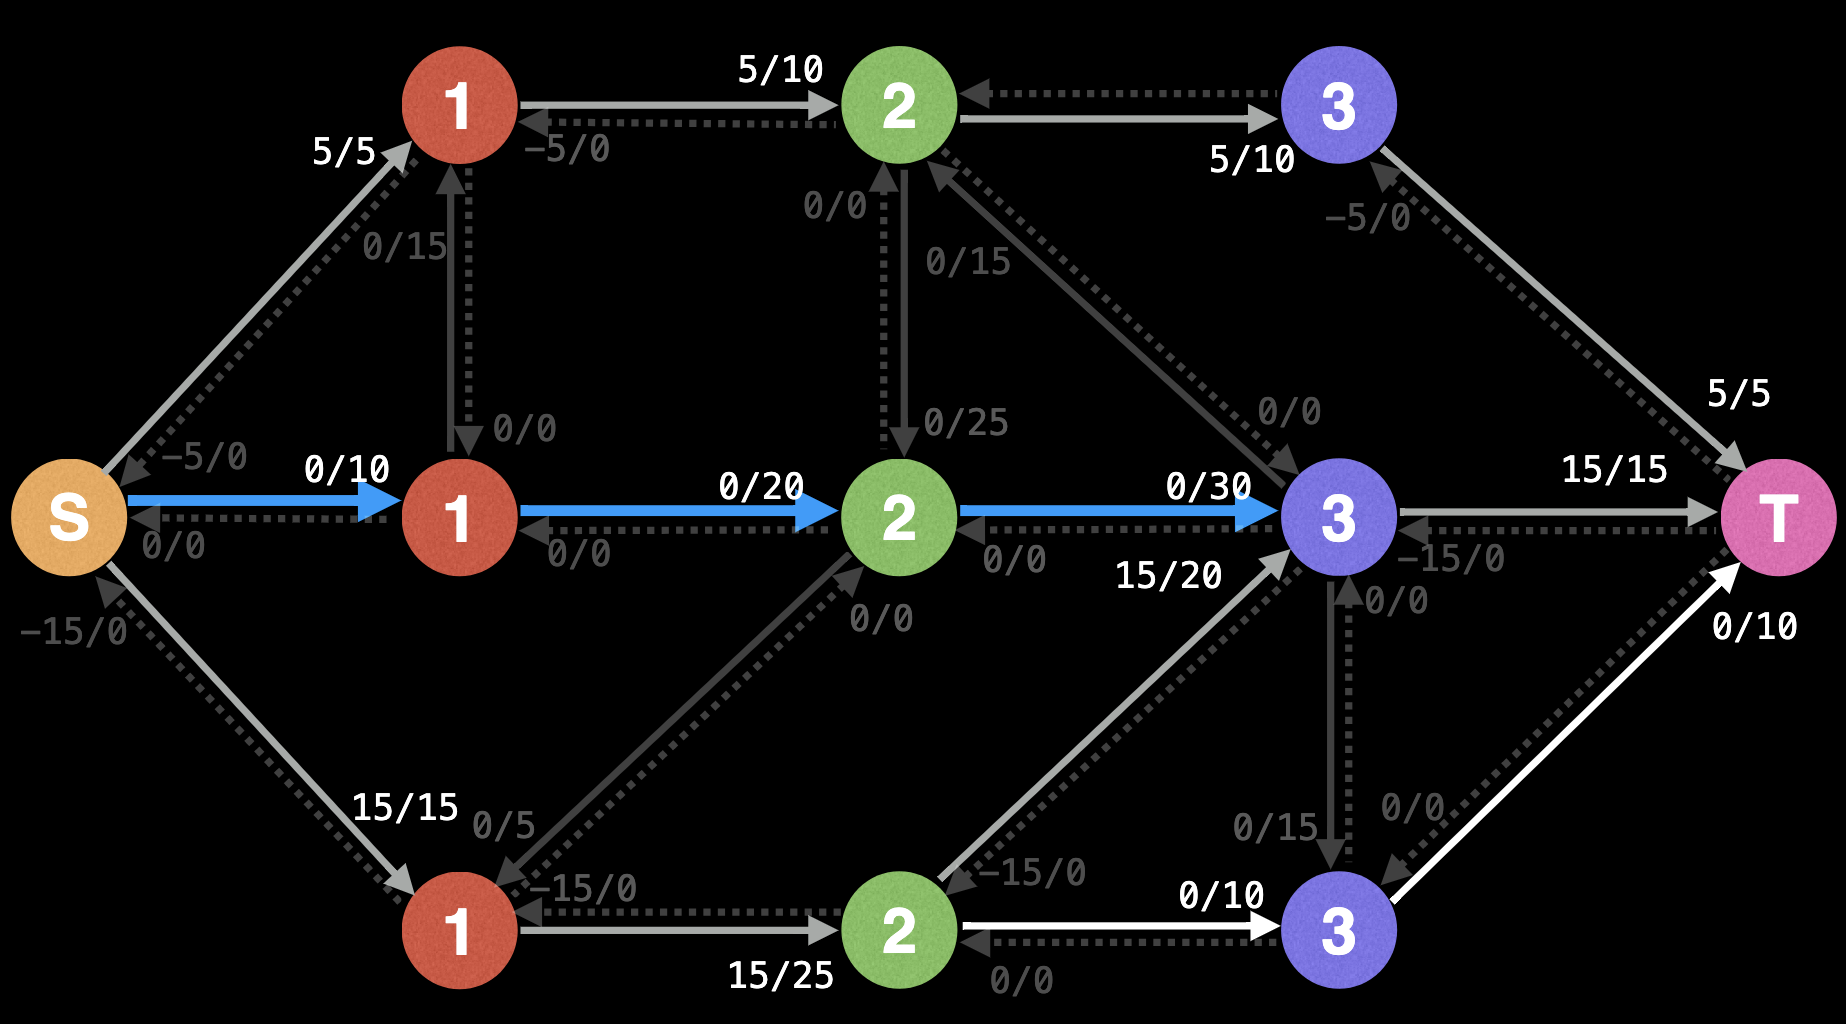
\includegraphics[width=\textwidth]{assets/visual07.png}
    \centering
    \captionsetup{justification=centering,margin=2cm}
    \caption{Blocking flow reached, so the algorithm has reached its end.}
\end{figure}
\begin{figure}[!htb]
    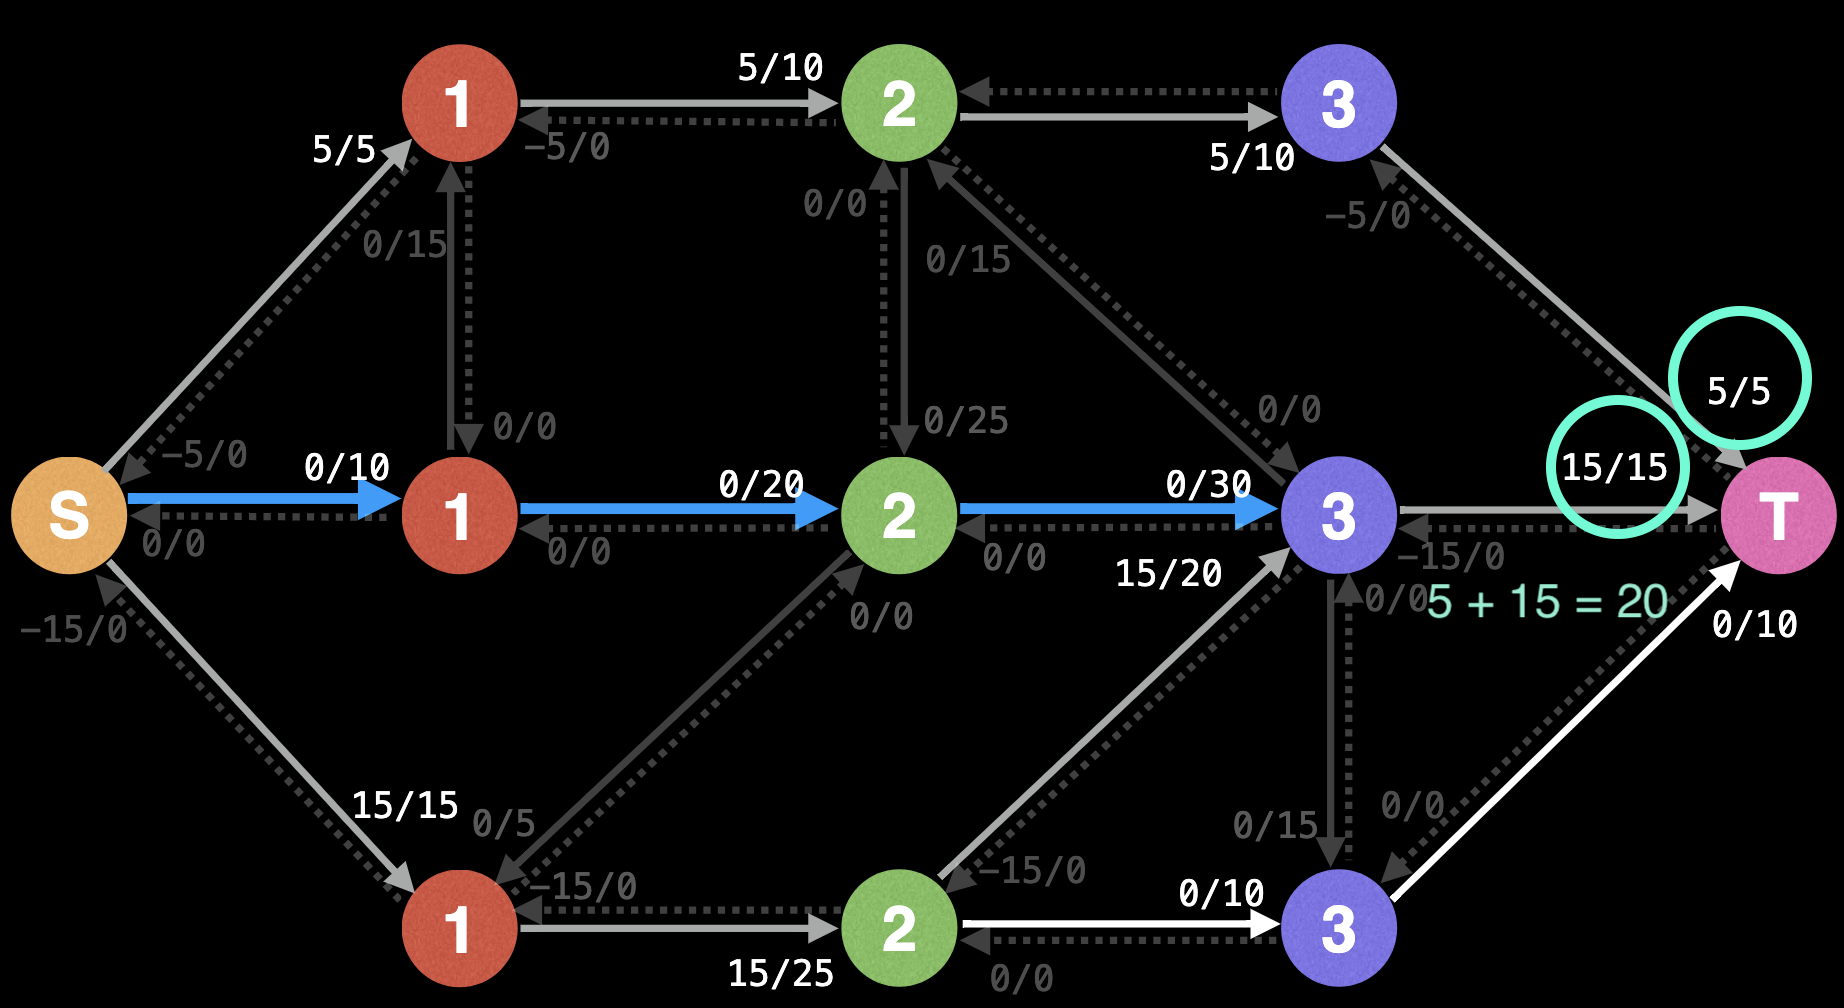
\includegraphics[width=\textwidth]{assets/visual08.png}
    \centering
    \captionsetup{justification=centering,margin=2cm}
    \caption{Maximum flow is the sum of the bottleneck values, so $5 + 15 = 20$.}
\end{figure}
\pagebreak

\section{Pseudo Code for Dinic's}
The following section contains a pseudo code example of how an implementation of the algorithm can be accomplished.

\makeatletter
\def\BState{\State\hskip-\ALG@thistlm}
\makeatother

\begin{algorithm}
\caption{Dinic's Algorithm}
\begin{algorithmic}[1]
\Procedure{BFS}{G, s} $\textit{G → graph, s → source}$
\State G.queue.push(s) $\textit{insert s in queue}$\\
\State \textbf{global} lvl = 1
\State s.lvl = lvl
\State s.visited = true\\
\BState \emph{while} G.queue is not empty:
\State{lvl += 1}
\State{v = G.queue.pop()}\\
\State{for each w $\in$ G.adj[s]}
\If {w is not visited}
\State G.queue.push(w)
\State {mark \textbf{w} as visited}
\State{w.lvl = lvl}
\EndIf\\
\EndProcedure\ {BFS}\\
\end{algorithmic}
\end{algorithm}

\begin{algorithm}
\begin{algorithmic}
\Procedure{DFS}{G, v, t, flow}
\If{v == sink \textbf{or not} flow}
\State{\textbf{return} flow}
\EndIf\\

\BState{\textbf{for} i \textbf{in} (v. . .sizeof(G.adj)):}
\State{edge = G.adj[v][i]}
\If{edge[0].lvl == v.lvl + 1}
\State{path = DFS(G, edge[0], t, min(flow, edge[2] - edge[3])}
\If{path}
\State{G.adj[v][i][3] += path}
\State{G.adj[edge[0]][edge[1]][3] -= path}
\State{\textbf{return} path}
\EndIf
\EndIf
\State{\textbf{return} 0}
\EndProcedure\ {DFS}\\

\Procedure{max\_flow}{G, s, t}
\State {BFS(G, s)}
\State{path\_flow = DFS(G, s, t, $\infty$)} $\textit{send infinite 'water' down the pipes}$
\BState{\textbf{while} path\_flow:}
\State{flow += path\_flow}
\State{path\_flow = DFS(G, s, t, $\infty$)}
\If{\textbf{not} t.lvl}
\State{\textbf{break}}
\EndIf
\State{\textbf{return} flow}
\EndProcedure\ MAX\_FLOW
\end{algorithmic}
\end{algorithm}



\chapter{Code Analysis}
This section of the document discusses the analysis of our algorithm including assessing both the time complexity and correctness of the algorithm. In the sections below the processes that were employed are described in detail. Additionally, the results will be provided in full.

\section{Time Complexity}
As previously mentioned in the report the time complexity of this algorithm is $O(|V|^2|E|)$. In order to confirm this our team created many random test cases where we controlled the number of nodes and edges in a weighted graph. However, it should be noted that we did not control whether these test cases connected the source and sink. This later became an issue when trying to analyze the results, but this will be discussed later. After generating each test case we ran the algorithm and recorded the number of nodes, edges, max flow (if any), and execution time of the algorithm in secs and stored these results in a text file. This was repeated a number of times while increasing the number of nodes and edges each time.

After enough iterations have been recorded the text file was imported into an excel sheet and the execution times were plotted on a scatter chart. An example of this chart can be seen below.

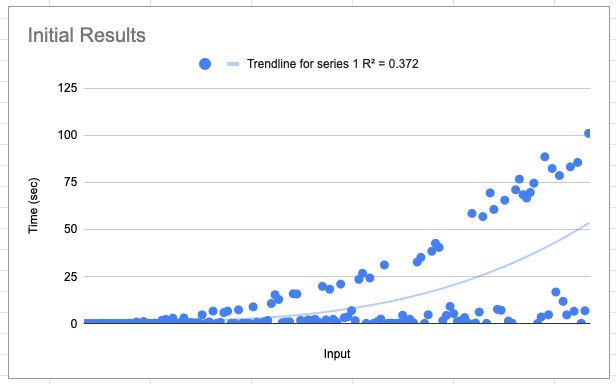
\includegraphics[width=\textwidth]{assets/Josh1.png}

What rapidly became apparent was that the data appeared to follow two different trends as the input was increased. We found that in these cases the max flow was consistently zero. The reason for this is because in these test cases the sink was not connected to the source which is the best case scenario for this algorithm so the execution time was consistently fast no matter the size of the input. In order to prevent this from skewing our r squared value we decided to exclude these results and simply plot only the execution times for the test cases where the sink and source were connected. This resulted in the following scatter plot:

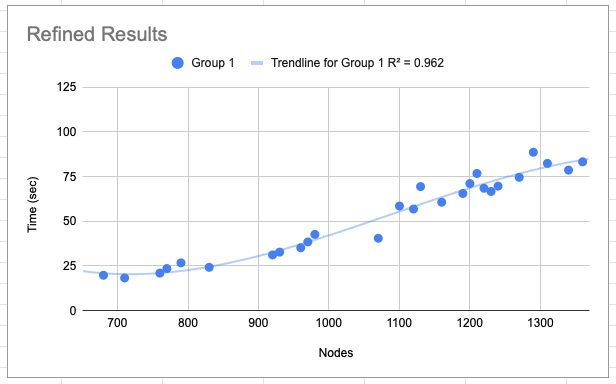
\includegraphics[width=\textwidth]{assets/Josh2.png}

Here, we saw that we got an excellent r squared value. This test was rerun a number of times using different test cases every time and the results were all similar so we concluded that our analysis of the algorithm's time complexity was correct.

\section{Correctness}
In addition to time complexity we also accessed our algorithm for correctness. Our test for correctness is relatively simple and far from complete by itself, but is of great importance to supporting our results for time complexity because if the algorithm isn't correct then the time complexity doesn’t matter.

With that said, to test correctness we simply found known test cases online and ran them through our algorithm to see if it produced the expected max flow. Below is an example of one test case that we found on GeeksforGeeks.

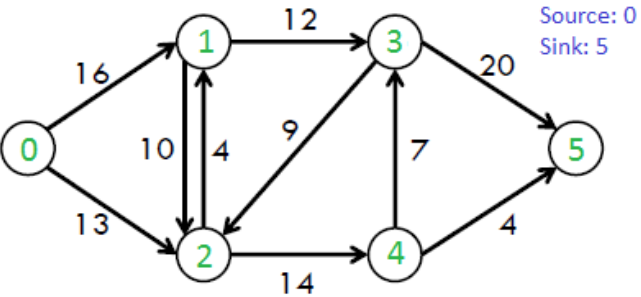
\includegraphics[width=\textwidth]{assets/Josh3.png}

Here you can see that the source is indeed connected to the sink and from the website we knew that the maxflow for this particular graph should be 23 and that is exactly what we got after running it through the algorithm. Therefore, our practical analysis is complete.

\chapter{Mathematical Analysis}
In this section, we will rigorously analyze Dinic's algorithm mathematically. First, we will provide some mathematical definitions that will be needed in order to formally define the algorithm. In the next section, we will attempt to formally define the algorithm using our definitions. The third section will feature analysis that establishes that Dinic's algorithm will find the max flow. The final section will analyze the time complexity of the algorithm.
\section{Some Definitions}
We first provide a formal definition of a network, which is the graph that we want to find the max flow of. We note that a network modifies a normal graph by adding capacities at every edge as well as defining a source and a sink node.
\begin{definition}[Network]
    We define a \textbf{network} by the tuple $(V, E, c, s, t)$ where:
    \begin{itemize}
        \item $V$ is a set of the vertices in the graph.
        \item $E$ is the set of the direct edges in the graph. We denote an edge between $u, v \in V$ by $u \rightarrow v$ or $(u \rightarrow v)^R$. We say that $G$ does not have multiple edges if it has no edges of the form $(u \rightarrow v)^R$.
        \item $c : E \mapsto \mathbb{N}$ is called the capacity function of the graph.
        \item $s \in V$ is called the source of the graph.
        \item $t \in V$ is called the sink of the graph.
    \end{itemize}
\end{definition}

A flow function is a tool used to define the flow that has been sent through each edge in the graph. This then has a corresponding constant, which represents the actual amount of flow that has been sent through the graph.
\begin{definition}[Flow Function]\thlabel{flowfunction}
    We define $f : E \mapsto \mathbb{N}$ as a flow function of $G$ if it has the following properties:
    \begin{itemize}
        \item
            $$f(e) \le c(e) \quad \forall e \in E$$
        \item
            $$\sum_{(u \rightarrow v) \in E}f(u \rightarrow v) + \sum_{(u \rightarrow v)^R \in E}f((u \rightarrow v)^R) = \sum_{(v \rightarrow u) \in E}f(v \rightarrow u) + \sum_{(v \rightarrow u)^R \in E}f((v \rightarrow u)^R)$$
            $$\forall u \in V, u \ne s, u \ne t$$
        \item
            $$f(u \rightarrow s) = 0 \quad \forall (u \rightarrow s) \in E$$
            $$f((u \rightarrow s)^R) = 0 \quad \forall (u \rightarrow s)^R \in E$$
            $$f(t \rightarrow u) = 0 \quad \forall (t \rightarrow u) \in E$$
            $$f((t \rightarrow u)^R) = 0 \quad \forall (t \rightarrow u)^R \in E$$
    \end{itemize}
    We then denote $f_s \in \mathbb{N}$ as the flow of $G$ in relation to $f$ if
    $$f_s = \sum_{(s \rightarrow u) \in E}f(s \rightarrow u) + \sum_{(s \rightarrow u)^R}f((s \rightarrow u)^R)$$
\end{definition}

We can now define the max flow (which is the value of interest of the algorithm). It is simply the maximum flow value possible.
\begin{definition}[Max Flow]\thlabel{maxflow}
    We define the maximum flow of a network, $G$, as, given the set of all possible flow functions of $G$, the largest corresponding flow value of all of these functions.
\end{definition}

A residual network is a modified type of network that is derived from a network and a flow function. The idea is to represent two edges for each edge in the network: a forward edge and a back edge. The forward edge has a capacity defined by the capacity left after accounting for the flow. On the other hand, the back edge has a capacity defined by the flow on the edge in the network. This tool is necessary to run most max flow algorithms.
\begin{definition}[Residual Network]\thlabel{residualnetwork}
    We define the network, $G_f^R$, as the residual network of $G$, a network without multiple edges, in terms of $f$ as the tuple $(V, E_f^R, c_f^R, s, t)$ where:
    \begin{itemize}
        \item
            $$E_f^R = E \cup \{(v \rightarrow u)^R \mid (u \rightarrow v) \in E\}$$
        \item
            $c_f^R : E_f^R \mapsto \mathbb{N}$ is defined as:
            $$c_f^R(u \rightarrow v) = c(u \rightarrow v) - f(u \rightarrow v)$$
            $$c_f^R((v \rightarrow u)^R) = f(u \rightarrow v)$$
    \end{itemize}
\end{definition}

A path is a common idea in graph theory. A path is simply a walk down edges in the graph in order from one vertex to another. Then, we define a shortest path as a path with shortest possible length between two edges.
\begin{definition}[Path]\thlabel{path}
    We define $P$ as a path from $u$ to $v$ in $G$ by a sequence of edges $(e_1, e_2, ..., e_{n-1})$ with an associated sequence of vertices $(v_1, v_2, ..., v_n)$ such that $e_i = (v_i \rightarrow v_{i+1})$, $e_i = (v_i \rightarrow v_{i+1})^R$, and $c(e_i) > 0$. It must also be the case that $v_1 = u$ and $v_n = v$. We call the value $n$ the length of the path.\\
    We call $P$ the shortest path from $u$ to $v$ if, when considering the all paths from $u$ to $v$, the length of $P$ is smaller or equal to the length of every other path.
\end{definition}

One can imagine a blocking flow as a flow function in the graph that forces the source to be disconnected from the sink in the residual graph. Hence, if a flow function is a blocking flow, no more flow can be sent through the graph.
\begin{definition}[Blocking Flow]\thlabel{blockingflow}
    We define $f$ as a blocking flow of a network $G$ if, for every path from $s$ to $t$ in $G$, there exists an edge, $e$, in the path such that $f(e) = c(e)$.
\end{definition}

A level function is simply a function that maps each vertex to its distance from the source node in a network.
\begin{definition}[Level Function]\thlabel{levelfunction}
    We define $l: v \mapsto \mathbb{N}$ as the level function of $G$ such that $l(v)$ is defined as the length of the shortest path from $s$ to $v$.
\end{definition}

A layered network is a another network that can be created by modifying another network. This takes a network and only includes edges where the level function increases by one along the edge. Hence, every path in a layered network will get further away from the source by one with each vertex.
\begin{definition}[Layered Network]\thlabel{layerednetwork}
    We define the network, $G^L$, as the layered network of $G$ with a level function $l$ by the tuple $(V, E^L, c^L, s, t)$ where:
    \begin{itemize}
        \item
            $$E^L = \{(u \rightarrow v) \mid (u \rightarrow v) \in E, l(u) = l(v) - 1\} \cup \{(u \rightarrow v)^R \mid (u \rightarrow v)^R \in E, l(u) = l(v) - 1\}$$
        \item
            $c^L : E \mapsto \mathbb{N}$ where $c^L(e) = c(e)$ if $e \in E^L$ and $c^L(e) = 0$ if $e \not\in E^L$.
    \end{itemize}
\end{definition}

\section{The Algorithm}
We will know propose the mathematical algorithm that will be used to compute the maximum flow of a graph. We consider the network $G = (V, E, c, s, t)$ to not have multiple edges and be constant throughout this section.\\
We now define $F = (f_0, f_1, ..., f_{n-1})$ to be a sequence of flow functions of $G$. We let $f_0$ be the zero function. Then, we define the following algorithm to compute $f_{i+1}$ given $f_i$.
\begin{algorithm}
\caption{Computing $f_{i+1}$ given $f_i$}\label{alg:cap}
\begin{algorithmic}
    \State $G_i' \gets G_{f_i}^R$ \Comment Get residual network
    \State $G_i'' \gets (G_i')^L$ \Comment Get layered network
    \State $f_i' \gets$ a blocking flow of $G''$
    \State $f_{i+1}(u \rightarrow v) \gets f_i(u \rightarrow v) + f_i'(u \rightarrow v) - f_i'((v \rightarrow u)^R)$ \Comment Update flow
\end{algorithmic}
\end{algorithm}
This represents the basic structure of the algorithm. Thus, the remaining mathematical analysis will focus on proving the correctness and complexity of the algorithm. To do this, we will conclude the following two things:
\begin{itemize}
    \item
        The flow of $G$ in relation to $f_{n-1}$ is the maximum flow of $G$.
    \item
        Using this algorithm, we can find the maximum flow in $O(|V|^2|E|)$ time.
\end{itemize}

\section{Correctness}
The following is a proposition; the proof of this has been omitted. This fact is used for most algorithms that find the max flow of a network. For the sake of this paper, the proof was ommitted for brevity.
\begin{proposition}\thlabel{prop1}
    Let $f$, $f'$ be flow functions of $G$. Let $f_s$, $f_s'$ be their corresponding flows. If $f_s' < f_s$, then there exists a path from $s$ to $t$ in $G$, $P$, such that:
    $$f'(e) > f(e) \quad \forall e \in P$$
\end{proposition}

This lemma features the fundamental fact that blocking flows are analogous to the max flow. This allows for the problem to be changed from finding the max flow to finding a blocking flow.
\begin{lemma}\thlabel{lemma1}
    Let $f$ be a blocking flow function of $G$. Let $f_s$ be the corresponding flow of $f$. Then, $f_s$ is the max flow of $G$.
\end{lemma}
\begin{proof}
    Assume that $f_s$ is not the max flow of $G$ for the sake of reaching a contradiction. Let $f'$ be a flow function of $G$ where its corresponding flow, $f_s'$, is the max flow of $G$. By our assumption, $f_s' > f_s$. Then, by Proposition \ref{prop1}, there is a path, $P$, from $s$ to $t$ such that:
    $$f'(e) > f(e) \quad \forall e \in P$$
    Because $f$ is a blocking flow, there is a $e_0 \in P$ such that $f(e_0) = c(e_0)$. Therefore, $f'(e_0) > c(e_0)$. Hence, $f'$ cannot be a valid flow function of $G$. Our assumption that $f_s$ is not the max flow of $G$ has caused us to reach a contradiction, which means that $f_s$ must be the max flow of $G$.
\end{proof}

This is another important lemma, and it proves that each $f_i$ found by the algorithm is a flow function. This is important because in order for the final flow function to be a blocking flow, it must first be a flow function.
\begin{lemma}\thlabel{lemma2}
    If $0 \le i < n$, then $f_i$ is a flow function of $G$.
\end{lemma}
\begin{proof}
    We will proceed with this proof by induction:\\
    \textbf{Base Case}:\\
    We note that the function $f_0$ is the zero function. It can be trivially confirmed that the zero function is a valid flow function of $G$.\\
    \textbf{Inductive Case}:\\
    We will assume that $f_i$ is a flow function of $G$, and we will show that $f_{i+1}$ is also a flow function of $G$. We note that $f_i'$ is a flow function of $G''$. We will analyze each property of a flow function:
    \begin{enumerate}
        \item
            Let $(u \rightarrow v) \in E$ be arbitrary. Then, we know that:
            $$f_{i+1}(u \rightarrow v) = f_i(u \rightarrow v) + f_i'(u \rightarrow v) - f_i'((u \rightarrow v)^R)$$
            And, based on the definition of residual networks, we can derive that:
            $$f_i'(u \rightarrow v) \le c(u \rightarrow v) - f_i(u \rightarrow v)$$
            $$f_i'((u \rightarrow v)^R) \le f_i(u \rightarrow v)$$
            This means that:
            $$f_{i+1}(u \rightarrow v) \le c(u \rightarrow v) - f_i(u \rightarrow v)$$
            Because $f_i$ is a flow function, $f_i(u \rightarrow v) \ge 0$. This means that:
            $$f_{i+1}(u \rightarrow v) \le c(u \rightarrow v)$$
        \item
            Let $u \in V$ be arbitrary. Then,
            $$\sum_{(u \rightarrow v) \in E}f_{i+1}(u \rightarrow v) = \sum_{(u \rightarrow v) \in E}f_i(u \rightarrow v) + \sum_{(u \rightarrow v) \in E}f_i'(u \rightarrow v) - \sum_{(u \rightarrow v) \in E}f_i'((v \rightarrow u)^R)$$
            $$=\sum_{(u \rightarrow v) \in E}f_i(u \rightarrow v) + \left[ \sum_{(u \rightarrow v) \in E}f_i'(u \rightarrow v) + \sum_{(v \rightarrow u) \in E}f_i'((u \rightarrow v)^R) \right]$$
            $$- \sum_{(u \rightarrow v) \in E}f_i'((v \rightarrow u)^R) - \sum_{(v \rightarrow u) \in E}f_i'((u \rightarrow v)^R)$$
            $$=\sum_{(v \rightarrow u) \in E}f_i(v \rightarrow u) + \left[ \sum_{(v \rightarrow u) \in E}f_i'(v \rightarrow u) + \sum_{(u \rightarrow v) \in E}f_i'((v \rightarrow u)^R) \right]$$
            $$- \sum_{(u \rightarrow v) \in E}f_i'((v \rightarrow u)^R) - \sum_{(v \rightarrow u) \in E}f_i'((u \rightarrow v)^R)$$
            $$= \sum_{(v \rightarrow u) \in E}f_i(v \rightarrow u) + \sum_{(v \rightarrow u) \in E}f_i'(v \rightarrow u) - \sum_{(v \rightarrow u) \in E}f_i'((u \rightarrow v)^R)$$
            $$= \sum_{(v \rightarrow u) \in E}f_{i+1}(v \rightarrow u)$$
        \item
            First, let $(u \rightarrow s) \in E$ be arbitrary. Then, we know that $f_i(u \rightarrow s) = 0$. Consider:
            $$f_{i+1}(u \rightarrow s) = f_i(u \rightarrow s) + f_i'(u \rightarrow s) - f_i'((s \rightarrow u)^R)$$
            Because $f_i'$ is a flow function, $f_i'(u \rightarrow s) = 0$. We also note that $f_i'((s \rightarrow u)^R) = f_i(u \rightarrow s) = 0$. Hence, $f_{i+1}(u \rightarrow s) = 0$.
            Next, let $(t \rightarrow v) \in E$ be arbitrary. Then, we know that $f_i(t \rightarrow v) = 0$. Consider:
            $$f_{i+1}(t \rightarrow v) = f_i(t \rightarrow v) + f_i'(t \rightarrow v) + f_i'((v \rightarrow t)^R)$$
            Because $f_i'$ is a flow function, $f_i'(t \rightarrow v) = 0$. We also note that $f_i'((v \rightarrow t)^R) = f_i(t \rightarrow v) = 0$. Hence, $f_{i+1}(t \rightarrow v) = 0$.
    \end{enumerate}
    We have shown inductively that $f_i$ will satisfy all of the properties of a flow function of $G$.
\end{proof}

This is a helper function for the next lemma, and it simply states that if an edge exists in the residual of the $i$th iteration, then either that edge or its back edge must exist in the residual of the $i+1$th iteration.
\begin{lemma}\thlabel{lemma3}
    Let $c_i'$ be the capacity function of $G_i'$ and $c_{i+1}'$ be the capacity function of $G_{i+1}$. Let $(u \rightarrow v) \in E$ be arbitrary. Then, if $c_i'(u \rightarrow v) > 0$ or $c_i'((v \rightarrow u)^R) > 0$, then $c_{i+1}'(u \rightarrow v) > 0$ or $c_{i+1}'((v \rightarrow u)^R) > 0$.
\end{lemma}
\begin{proof}
    We will proceed with this proof by the contrapositive. We assume that $c_{i+1}'(u \rightarrow v) = 0$ and $c_{i+1}'((v \rightarrow u)^R) = 0$. Hence, we can conclude that $c(u \rightarrow v) = f_i(u \rightarrow v)$ and $f_i(u \rightarrow v) = 0$. Hence, $c(u \rightarrow v) = 0$. This means that $f_{i-1}(u \rightarrow v) = 0$ because $f_{i-1}$ is a flow function of $G$. Hence, we can conclude that $c_i'(u \rightarrow v) = 0$ and $c_i'((v \rightarrow u)^R) = 0$.
\end{proof}

This is another powerful lemma in the theory. This states that each node gets either further or stays the same distance away from the source node at each iteration's level graph. This will be very important in proving the next lemma.
\begin{lemma}\thlabel{lemma4}
    Let $v \in V$ be arbitrary. Let $l_i$ be the level function of $G_i'$ and $l_{i+1}$ be the level function of $G_{i+1}$. Then, $l_{i+1}(v) \ge l_i(v)$.
\end{lemma}
\begin{proof}
    Let $c_i'$ be the capacity function of $G_i$ and $c_{i+1}'$ be the capacity function of $G_{i+1}$. Let $P$ be a shortest path from $s$ to $v$ in $G_{i+1}'$. We will show that if $(u \rightarrow w) \in P$ or $((u \rightarrow w)^R) \in P$, then $l_{i+1}(w) \ge l_i(w)$ by induction:\\
    \textbf{Base Case}:\\
        We first note that $(s \rightarrow u)^R \not\in P$. Hence, we let $(s \rightarrow u) \in P$. This implies that $c_{i+1}'(s \rightarrow u) > 0$. We will now show that $c_i'(s \rightarrow u) > 0$. We first note the following properties:
        $$c_{i+1}'(s \rightarrow u) = c(s \rightarrow u) - f_{i+1}(s \rightarrow u)$$
        $$f_{i+1}(s \rightarrow u) = f_i(s \rightarrow u) + f_i'(s \rightarrow u) - f_i'((u \rightarrow s)^R)$$
        Because $f_i'((u \rightarrow s)^R) = 0$, $f_{i+1}(s \rightarrow u) \ge f_i(s \rightarrow u)$. We can then conclude that $c_{i+1}'(s \rightarrow u) \le c_i'(s \rightarrow u)$. Because $c_{i+1}'(s \rightarrow u) > 0$, $c_i(s \rightarrow u) > 0$. From this, we can conclude that $l_i(u) = l_{i+1}(u) = 1$.\\
    \textbf{Inductive Case}:\\
        Let $(u \rightarrow w) \in P$ or $(u \rightarrow w)^R \in P$. By the inductive hypothesis, we know that $l_{i+1}(u) \ge l_i(u)$. Because $P$ is a shortest path, $l_{i+1}(w) = l_{i+1}(u) + 1$. We will now consider two cases:
        First, we assume that $c_i'(u \rightarrow w) > 0$. In this case, $l_i(w) \le l_i(u) + 1$, which allows us to conclude that:
        $$l_i(w) \le l_i(u) + 1 \le l_{i+1}(u) + 1 = l_{i+1}(w)$$
        We now consider the case where $c_i'(u \rightarrow w) = 0$. We again split the problem into two cases:
        \begin{enumerate}
            \item
                We first assume that $(u \rightarrow w) \in P$. In this case, $c(u \rightarrow w) = f_i(u \rightarrow w)$. Because $c_{i+1}'(u \rightarrow w) > 0$, $c(u \rightarrow w) > f_{i+1}(u \rightarrow w)$. We can therefore conclude that $f_i'((w \rightarrow u)^R) > f_i'(u \rightarrow w) \ge 0$. Because $f_i'$ is the flow through the layered network, $l_i(u) = l_i(w) + 1$. we can now conclude:
                $$l_{i+1}(u) \ge l_i(w) + 1 \Rightarrow l_{i+1}(w) - 1 \ge l_i(w) + 1 \Rightarrow l_{i+1}(w) \ge l_i(w)$$
            \item
                Next, we assume that $(u \rightarrow w)^R \in P$. This means that $f_i(w \rightarrow u) = 0$. Because $c_{i+1}((u \rightarrow w)^R) > 0$, $f_{i+1}(w \rightarrow u) > 0$. From this, we conclude that, $f_i'(w \rightarrow u) > f_i'((u \rightarrow w)^R) \ge 0$. Because $f_i'$ is a blocking flow of the layered network, $l_i(w) + 1 = f_i(u)$. From this, we can conclude that:
                $$l_{i+1}(u) \ge l_i(w) + 1 \Rightarrow l_{i+1}(w) - 1 \ge l_i(w) + 1 \Rightarrow l_{i+1}(w) \ge l_i(w)$$
        \end{enumerate}
        In either case, we find that $l_{i+1}(w) \ge l_i(w)$.\\
    For some $u$, there must exist an edge from $u$ to $v$ in $P$. From this fact, we can conclude that $l_{i+1}(v) \ge l_i(v)$.
\end{proof}

This lemma represents the final step needed before showing completeness. We use the results from the last lemma to show that the sink vertex gets strictly further from the source vertex for each iteration. The true power of this lemma will be shown in the following theorem.
\begin{lemma}\thlabel{lemma5}
    Let $l_i$ be the level function of $G_i'$ and $l_{i+1}$ be the level function of $G_{i+1}'$. Then, $l_{i+1}(t) > l_i(t)$.
\end{lemma}
\begin{proof}
    Lemma \ref{lemma4} states that $l_{i+1}(t) \ge l_i(t)$. Let us assume that $l_{i+1}(t) = l_i(t)$ for the sake of reaching a contradiction. Let P be a shortest path from $s$ to $t$ in $G_{i+1}'$. $P$ must also be a shortest path from $s$ to $t$ in $G_i'$. Because $f_i'$ is a blocking flow of $G_i''$, there is an $e \in P$ such that $f_i'(e) = c_i'(e)$. Now, we will consider two cases:
    \begin{enumerate}
        \item
            If

 $e$ has the form $u \rightarrow w$. Now, we conclude that:
            $$f_{i+1}(u \rightarrow w) = f_i(u \rightarrow w) + f_i'(u \rightarrow w) - f_i'((w \rightarrow u)^R)$$
            $$= f_i(u \rightarrow w) + c_i'(u \rightarrow w) - f_i'((w \rightarrow u)^R)$$
            $$= f_i(u \rightarrow w) + c(u \rightarrow w) - f_i(u \rightarrow w) - f_i'((w \rightarrow u)^R)$$
            $$= c(u \rightarrow w) - f_i'((w \rightarrow u)^R)$$
            We can conclude that $f_i'(u \rightarrow w) > 0$. We conclude from this that $l_i(u) + 1 = l_i(w)$. Hence, we know that $f_i'((w \rightarrow u)^R)$. Then, we conclude that $c_{i+1}'(u \rightarrow w) = 0$. This is a contradiction because $P$ is a path in $G_i'$.
        \item
            Assume that $e$ has the form $(u \rightarrow w)^R$. Following similar logic to the previous case, we conclude that:
            $$f_{i+1}(w \rightarrow u) = f_i(w \rightarrow u) + f_i'(w \rightarrow u) - c_i'((u \rightarrow w)^R) = f_i'(w \rightarrow u)$$
            From this, we conclude that $c_{i+1}'((u \rightarrow w)^R) = 0$, which is also a contradiction
    \end{enumerate}
    In either case we reach a contradiction. Hence, $l_{i+1}(t) \ne l_i(t)$. We can now conclude that $l_{i+1}(t) > l_i(t)$.
\end{proof}

This theorem is the puzzle piece that shows the completeness of the algorithm. Through this, we know that the algorithm is able to terminate in a finite number of steps. Not only this, but we know that it reaches a blocking flow! Because a blocking flow is also a max flow, this algorithm solves the  problem and is able to find the max flow of the network.
\begin{theorem}\thlabel{theorem1}
    There is a finite $n$ such that $f_n$ is a blocking flow of $G$.
\end{theorem}
\begin{proof}
    We first note that, if $l$ is a level function of a network with $V'$ as its set of vertices, $l(v) \le |V'|$, where $v \in V'$. We now use the notation that $l_i$ is the level function of $G_i'$. By Lemma \ref{lemma5}, $l_{i+1}(t) > l_i(t)$. This means that $l_i(t) \ge i$. From this, we can conclude that $l_{|V'|}(t) \ge |V'|$. Hence, $n \le |V'|$.
\end{proof}

\section{Complexity}
In order to establish the complexity, we must analyze many of the different individual parts of the algorithm. First, in the next lemma, we will show that if we have a layered network, we can compute its blocking flow in $O(|V||E|)$ time.
\begin{lemma}\thlabel{lemma6}
    Let $G^L$ be a layered network with a level function, $l$. Then, we can find a blocking flow function, $f$, in $O(|V||E|)$ time.
\end{lemma}
\begin{proof}
    The process of finding a blocking flow function is done by finding every path from $s$ to $t$ in $G^L$ and doing the following:
    \begin{enumerate}
        \item Updating the blocking flow along the path.
        \item Updating capacities along the path
        \item Removing an edge along the path
    \end{enumerate}
    Hence, the number of paths that we explore must be less than $|E|$. Now, we must compute how long it takes to explore a path. Because the length of a path is at maximum $|V|$, we can update the blocking flows and capacities in $O(|V|)$ time in the worst case. Now, we can declare a function, $n : V \mapsto V$, which maps the next node in a path from the previous node. This value can be trivially updated after an edge removal. Hence, a path can be found in $O(|V|)$ time. Because there are $O(|E|)$ paths to explore, it takes $O(|V||E|)$ time to find $f$.
\end{proof}

Next, we use the previous lemma to create a more powerful result. If we have the $i$th flow function, we can compute the $i+1$th flow function in $O(|V||E|)$ time.
\begin{lemma}\thlabel{lemma7}
    Suppose we know $f_i$ for $G$. We can derive $f_{i+1}$ in $O(|V||E|)$ time.
\end{lemma}
\begin{proof}
    First, $G'_i$ can be derived from $G$ by iterating over the edges in $G$ in $O(|E|)$ time. Then, $G''_i$ can be derived from $G'_i$ by using a BFS traversal of $G'_i$, which can be computed in $O(|E|)$ time (we assume here that $|E| > |V|$). Then, $f_i'$ can be derived in $O(|E||V|)$ time using Lemma \ref{lemma6}. Finally, we can compute $f_{i+1}$ from $f_i'$ and $f_i$ by iterating over every edge in $O(|E|)$ time. This implies that we can find $f_{i+1}$ in $O(|E||V|)$ time.
\end{proof}

We now feature this theorem, which establishes the time complexity of the entire algorithm. Through this theorem, we show that we can find the maximum flow of a network in $O(|V|^2|E|)$ time.
\begin{theorem}\thlabel{theorem2}
    Given a network, $G$, we can find its maximum flow in $O(|V|^2|E|)$ time.
\end{theorem}
\begin{proof}
    We first note that $f_{i+1}$ can be derived from $f_i$ in $O(|V||E|)$ time using Lemma \ref{lemma7}. Theorem \ref{theorem1} tells us that $n \le |V|$. Hence, $f_n$ can be computed in $O(|V|^2|E|)$ time. We know that the flow of $f_n$ is the maximum flow of $G$. We can trivially find the flow value of $f_n$ in $O(|E|)$ time. Therefore, the maximum flow can be found in $O(|V|^2|E|)$ time.
\end{proof}

\chapter{Conclusions}

\end{document}
